\chapter{Geophysics Interferometer (GIF)} \label{chap3}
KAGRA is the only GW detector, which has a strainmeter to monitor its baseline length changes. The strainmeter is named Geophysics interferometer (GIF).

GIF is a laser interferometric strainmeter, which is developed by reserchers in Earthquake Research Institute, University of Tokyo. The purpose of the strainmeter is to observe geophysical phenomena: not only earthquakes but also Earth's free oscillations. Unlike a seismometer, the strainmeter has a sensitivity in low-frequency. Moreover, unlike the continuous GPS (CGPS) nets, which also measures a strain ($\sim\,10^{-8}$), the strainmeter has more precision ($\sim\,10^{-12}$) \cite{araya2007broadband}.

In this chapter, instruments of GIF are described. After overview of GIF in section \cref{sec:sec41}, working principles of the interferometer are described in section \cref{sec:sec42}. Optics of GIF are described in section \cref{sec:sec43}. Realtime signal aquisition system to send the strain signal to KAGRA is described in \cref{sec:sec44}

\section{Overview} \label{sec:sec41}
Geophysics interferometer (GIF) is a $1500\,\mathrm{m}$ laser strainmeter constructed parallel to X-arm baseline of KAGRA. As shown in Figure \ref{img:img402}, GIF is an asymmetric Michelson interferometer unlike symmetric KAGRA interferometer. Moreover, mirrors of the interferometer of GIF are fixed on the ground in order to monitor the baseline length changes directly. GIF is now only installed on the X-arm, which has been observing the baseline changes for almost 3 years.
\begin{figure}[h]
  \centering
  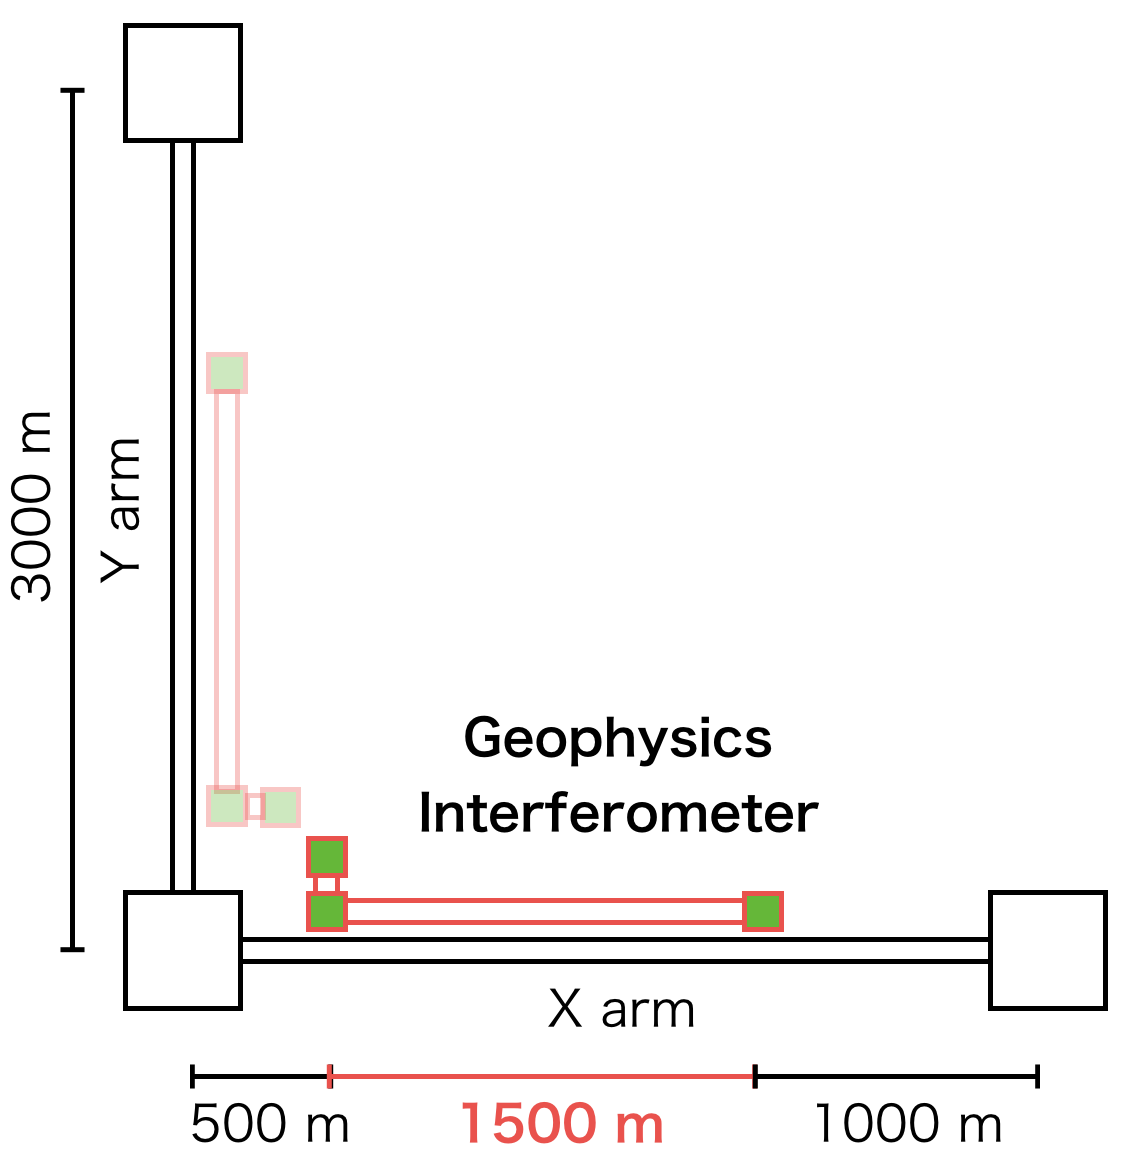
\includegraphics[width=8cm]{./img_chap4/img402.png}
  \caption{Location of geophysics interferometer (GIF). Whereas KAGRA is a symmetric L-shape $3000\,\mathrm{m}$ Michelson interferometer, GIF is an asymmetric $1500\,\mathrm{m}$ Michelson interferometer. GIF is only installed along the X-arm tunnel.} \label{img:img402}
\end{figure}

\section{Working Principle} \label{sec:sec42}
As described in section \cref{sec:12}, working principle of the strain measurement of GIF is the same as the GW detectors. However, the sensitivity of GIF is limited by the laser frequency noise due to the asymmetric optical configuration.
\subsection{Asymmetric Michelson Interferometer}
\begin{figure}[h]
  \centering
  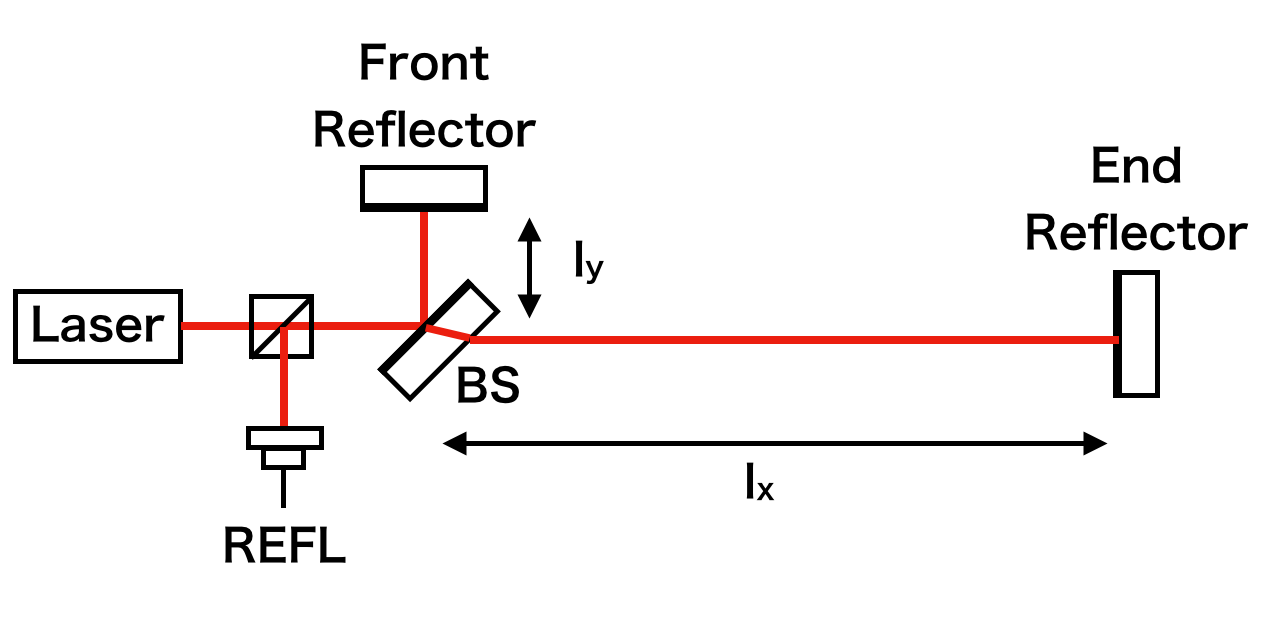
\includegraphics[width=10.0cm]{./img_chap4/img401.png}
  \caption{Schematic drawing of the GIF as an asymmetric Michelson interferometer, which has two different arm length, $l_x\gg{l_y}$. In this figure, the mode matching optics and the optics for signal detection are not drawn.} \label{img:img401}
\end{figure}
A schematic optical layout of the GIF interferometer as an asymmetric Michelson interferometer is shown in Figure  \ref{img:img401}. The asymmetric interferometer measure change of baseline length $l_x$ with reference to the short arm $l_y$, and its fringe signal is obtained at the REFL port in the case of the GIF.

Here, we consider how the asymmetric arms affect to the optical phase of the interferometer. The relation between of the optical phase $\phi_{-}$ and the differential of the arms length ${L_{-}}=l_{\mathrm{x}}-l_{\mathrm{y}}$ is given as ${\phi}_{-} = 4\pi\frac{{L_{-}}}{\lambda}$, where $\lambda$ is the wavelength of the laser. This relation introduce the relation of the infinitesimal changes between in these phsical parameters;
\begin{eqnarray}  
  \left|\Delta \phi_{-}\right| = \frac{4\pi{L_{-}}}{\lambda}\left( \left|\frac{\Delta L_{-}}{L_{-}}\right| + \left|\frac{\Delta f}{f}\right|\right), \label{eq:eq400}
\end{eqnarray}
where $\Delta$ denote the infinitesimal change of the parameters and $f$ if the frequency of the laser, and relation $|\frac{\Delta{\lambda}}{\lambda}| = |\frac{\Delta{f}}{f}|$ was used to represent with the frequency fluctuation. Assuming enough asymmetricity of each arm length $l_{\mathrm{x}} \gg l_{\mathrm{y}}$ and the short reference arm is the rigid bar $\Delta l_{\mathrm{y}} \ll 1$ (this assumption is true because the short arm of $l_y$ is made of the super-invar plate whose coefficient of thermal expansion is extremely low), Eq.(\ref{eq:eq400}) can be represented as
\begin{eqnarray}  
  \left|\Delta \phi_{-}\right| = \frac{4\pi{l_{\mathrm{x}}}}{\lambda}\left( \left|h\right|  + \left|\frac{\Delta f}{f}\right|\right), \label{eq:eq400_a}
\end{eqnarray}
where $h = \Delta{l_{x}}/l_x$ is the strain of the baseline. It is clear that the strain and the laser frequency fluctuation are the same response to the optical phase. In other words, the frequency noise directly affects to noise of the strain measurement.

\newpage
\subsection{Seismic Strain Response}
\begin{figure}[h]
  \centering
  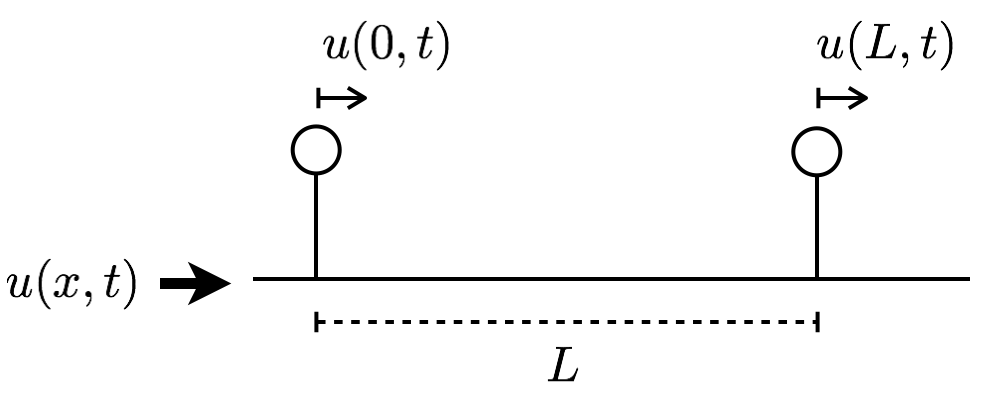
\includegraphics[width=10cm]{./img_chap4/img430.png}
  \caption{} \label{img:img430}
\end{figure}
Here, we consider the response from strain to the optical phase in the case that the plane seismic waves whose displacement $u(t,x)$ is represented as $u(t,x)=u_0e^{i(\omega{t}-kx)}$ with angular frequency of $\omega$ and the wavenumber of $k$. The seismic wave propagates along with the direction of the baseline of the strainmeter (right direction in this figure).

\subsubsection{Response from $u$ to $\Delta{L}$, ($H_{\mathrm{disp}}$)}
Before calculating the strain response, we calculate the response from the displacement of the seismic wave to the baseline length change. First, because the length fluctuation between two mirrors sparated with $L$ can be expressed as 
\begin{eqnarray} 
  \Delta{L(t)} &\equiv& u(t,0) - u(t,L) \\
  &=& u(t,0) - u(t-\tau,0), \label{eq:eq403}
\end{eqnarray}
where $\tau=L/v$ is the time delay, the transfer function from the displacement to the length fluctuation is given by Laplace transform as
\begin{eqnarray} \label{eq:eq404}
  H_{\mathrm{disp}}(s) \equiv \frac{\Delta{L(s)}}{u(s)} = \frac{u(s)\left[ 1-\exp(-\tau{s}) \right]}{u(s)} = 1 - \exp(-\tau{s})
\end{eqnarray}

\subsubsection{Response from $\epsilon$ to $\phi_{-}$, ($H_{\mathrm{strain}}$)}
Because the strain amplitude $\epsilon{(x,t)}$ is defined as $\epsilon{(x,t)}\equiv\frac{du}{dx}$, the seismic strain is represented as 
\begin{eqnarray} 
  \epsilon{(x,t)} \equiv \frac{du}{dx} = \frac{du}{dt} \frac{1}{v} = \frac{s}{v}u(s) \label{eq:eq406}
\end{eqnarray}
Therefore, the transfer function from the seismic strain to the displacement is given  as
\begin{eqnarray} \label{eq:eq407}
  \frac{\Delta{L(s)}}{\epsilon(s)} = H_{\mathrm{disp}} \frac{v}{s}
\end{eqnarray}
Finally, because the transfer function from the length change of the baseline to the optical phase is given as $4\pi/{\lambda_{\mathrm{opt}}}$, the transfer function from the seismic strain to the optical phase is represented as 
\begin{eqnarray} \label{eq:eq407}
  H_{\mathrm{strain}}(s) = 4\pi\frac{1}{\lambda_{\mathrm{opt}}} \left[1 - \exp(-\tau{s}) \right]\frac{v}{s}.
\end{eqnarray}

Here, as a summary of these transfer function, these are related with each other as shown in Figure (\ref{img:img411}). 

\begin{figure}[h]
  \centering
  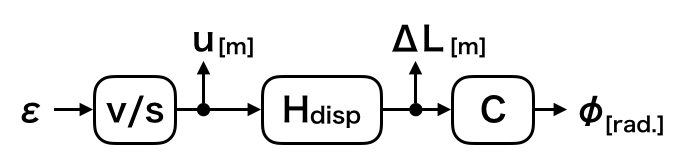
\includegraphics[width=10.0cm]{./img_chap4/img411.png}
  \caption{The response from seismic strain to optical phase.} \label{img:img411}
\end{figure}

\subsubsection{Improvement of the sensitivity with longer baseline}
Here, we describe the length dependance of the strain response given by Eq.(\ref{eq:eq407}). Bode plot of the strain response with two different baseline length is shown in Figure  \ref{img:img411_a}, in the case that the phase velocity is $5.5\,\mathrm{km}$. One can find that the DC gain is greater for $L=3000\,\mathrm{m}$ than the gain for $L=3000\,\mathrm{m}$, and the corner frequency is lower in the case of long baseline.

Because the corner frequency $f_0\equiv {1}/{\tau}$ is given as
\begin{eqnarray}
  f_0 = \frac{v}{L},
\end{eqnarray}
if the baseline length is twice, the frequency is half, which means decrease of the observation frequency band. For example, in the case of $L=1500\,\mathrm{m}$, and assuming the phase velocity of $5.5 \mathrm{km/sec}$, the corner frequency is $f_0\sim3.7\,\mathrm{Hz}$. Below this frequency, therefore, the GIF interferometer responses the strain as the flat response.

\begin{figure}[p]
  \begin{center}
    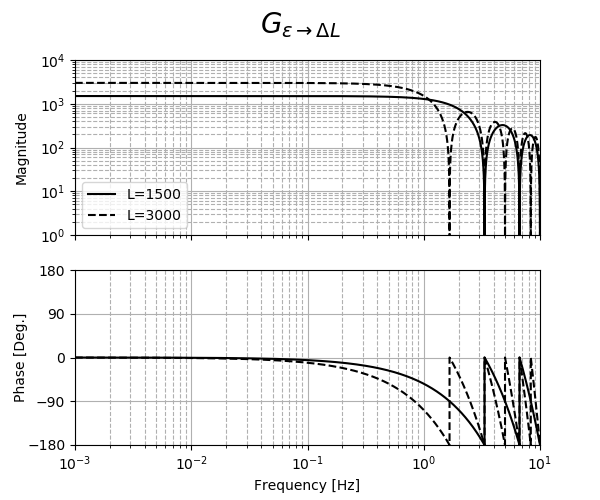
\includegraphics[width=13.0cm]{./img_chap4/img412.png}
    \caption{Compasison of the transfer function from strain of the baseline $\epsilon$ to the length change of that $\Delta{L}$ in the different baseline length.}\label{img:img411_a}
  \end{center}
\end{figure}

\subsection{Noise}
\subsubsection{Frequency Noise} \label{sec:123}
As mentioned above, the noise of asymmetric interferometer is limited by the frequency noise because the commom mode rejection was not work sufficiently. The GIF, therefore, use the frequency stabilized laser by using iodine-absorption line \cite{araya2017design}. The fluctuation $\Delta{f}/f$, which coresponds to the stain, is
\begin{eqnarray}
  h = \frac{\Delta{f}}{f} \sim 7\times10^{-13} [\mathrm{1/\mathrm{Hz}}].
\end{eqnarray}

\subsubsection{Residual Gas Noise}
Bcause residual gas fluctuates the optical path, length measured by interferometer is also fluctuates. The opttical path $L_{\mathrm{opt}}$ is given by $L_{\mathrm{opt}}=nL$, where $L$ is the length of the baseline and $n$ is the refraction index in the optical path relative to the path in the vacuum. Under the pressure of $p$ in vacuum, the index $n$ is approximated as $n = 1 + c_0(p/p_0)$, where $c_0$ denotes the relattive refractive index, $p_0$ is pressure in standard air at 1 atm. The apparent strain due to the residual pressure is given as \cite{ciddor1996refractive};
\begin{eqnarray}
  h = (L_{\mathrm{opt}}-L)/L = c_0(p/p_0) \sim 3\times10^{-9} p.
\end{eqnarray}
In order to maintain the strain sensitivity; $3\times10^{-13}$, the vacuum pressure should be below $1\times10^{-4}\,[\mathrm{Pa}]$. However, actual vacuum pressure is $1\times10^{-2}\,[\mathrm{Pa}]$, then strain is $\sim\times10^{-12}$.


\section{Optics} \label{sec:sec43}
In preivious discussion, the laser light was implicitly assumed the plane wave, which does not change the optical phase and radius of the beam when it propagates, but actual beam is not. The actual beam requires a design of these beam profiles to interfer the beam within a finite scale. In this section, we assume a Gaussian beam, and describe the design for the GIF interferometer.

\subsection{Gaussian Beam}
\subsubsection{Gaussian beam}
Ideal Gaussian beam has the fundamental spatial mode called $\mathrm{TEM}_{00}$. The whose electric field of the beam propagating to $z$ axis is given by \cite{bond2016interferometer,svelto1998principles}
\begin{eqnarray}
  u(x, y, z)=\sqrt{\frac{2}{\pi{w^2(z)}}} \exp \left(i\zeta(z)-\mathrm{i} k \frac{x^{2} +y^{2}}{2 R(z)}-i\frac{2\pi}{\lambda}z\right)
  \exp \left(-\frac{x^{2}+y^{2}}{w^{2}(z)}\right),  \label{eq:eq415}
\end{eqnarray}
where $\lambda,\,w_0$ are the wavelength and the beam radius at $x=0$ of the beam. In addition,
\begin{eqnarray}
  z_0 &=& \frac{\pi{w^2_0}}{\lambda} \\ \label{eq:eq415_a}
  w(z) &=& w_0\sqrt{1+\left(\frac{z}{z_0}\right)^2}, \\ \label{eq:eq415_b}
  R(z) &=& z\left[1+\left(\frac{z_0}{z}\right)^2\right],\\ \label{eq:eq415_c}
  \phi(z) &=& \arctan\left(\frac{z}{z_0}\right) \label{eq:eq415_d}
\end{eqnarray}
are Reyliegh range and radius, curvature, and Gouy phase of the beam as a function of $z$, respectively. One can find that power of the beam $|u^2|$ has a Gaussian distribution as shown in Figure  \ref{img:img415a} according to Eq.(\ref{eq:eq415}). 

\begin{figure}[p]
  \begin{minipage}{14cm}
    \centering    
    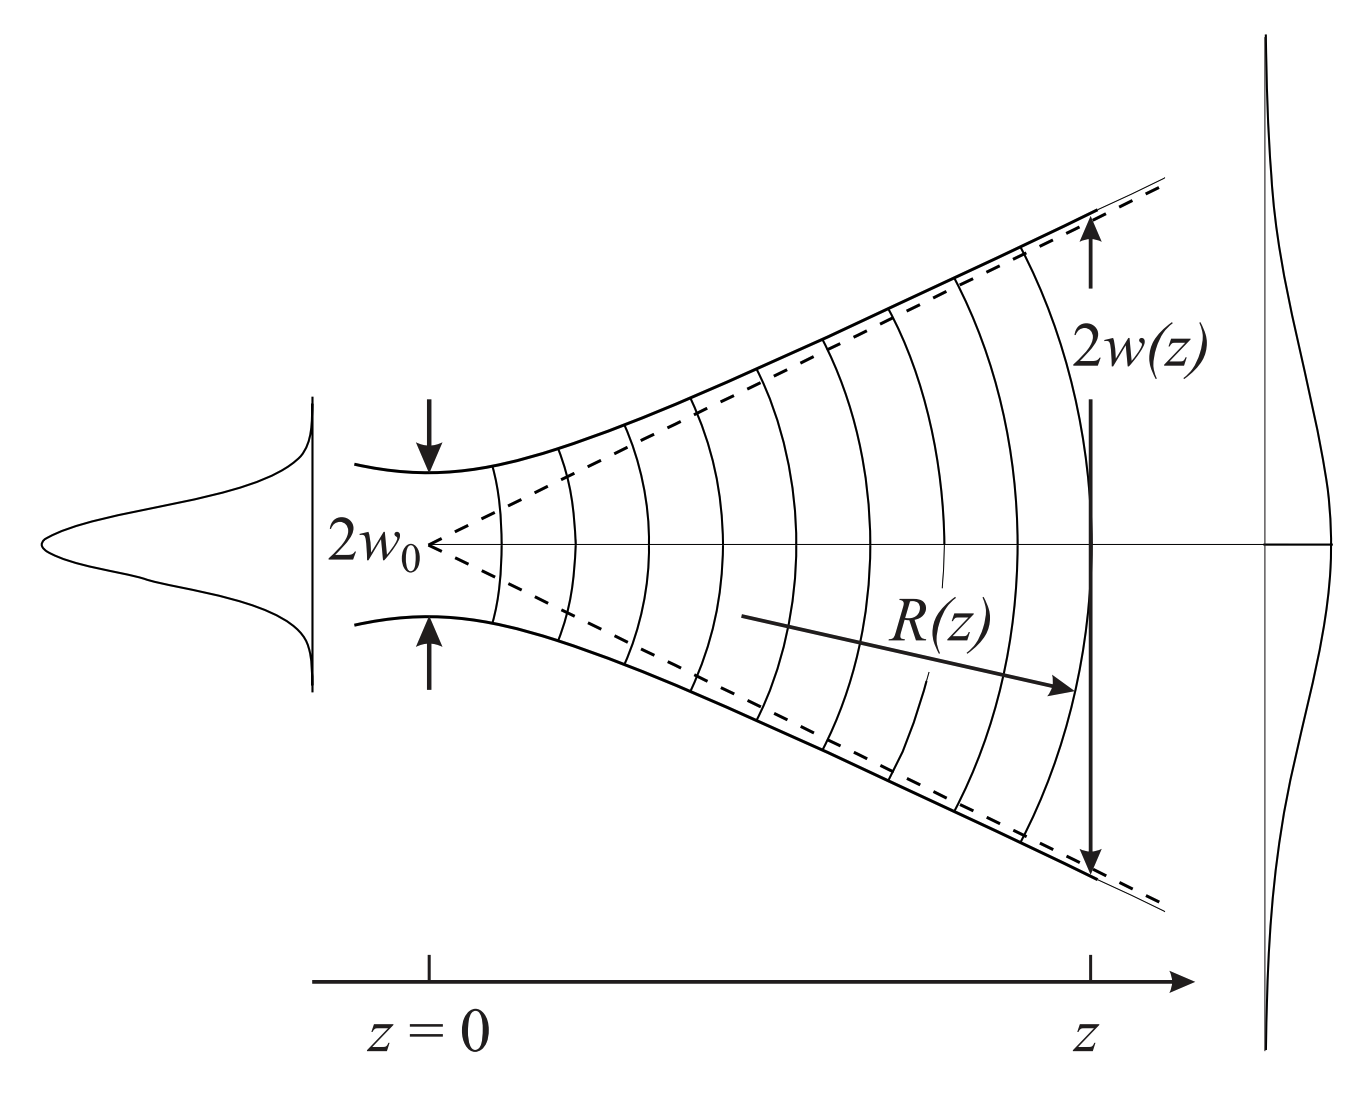
\includegraphics[width=8cm]{./img_chap4/img415a.png}
    \subcaption{Evolution of a Gaussian beam propagating along the z-axis\cite{riehle2006frequency}}{$w_0$ denotes a beam radius at beam weist, where $z=0$. $w(z)$ and $R(z)$ are the beam radius and curvature at $z$. Gouy phase is not shown in here.}\label{img:img415a}
  \end{minipage}\\
  \begin{minipage}{14cm}
    \centering        
    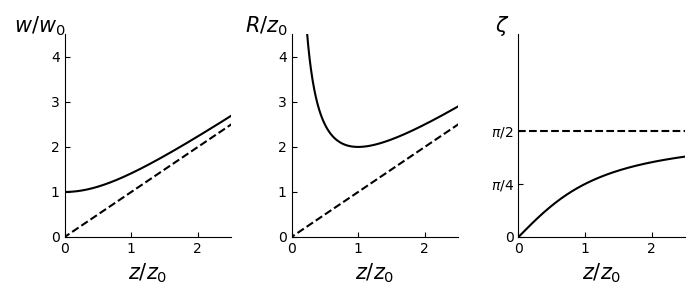
\includegraphics[width=14cm]{./img_chap4/img415.png}
    \subcaption{Beam prifile}{(left) Beam radius normalized by $w_0$ as a function of $z/z_0$, where $z_0$ is Rayleigh length. (Middle) Beam curvature normalized by $z_0$. (right) Gouy phase.}\label{img:img415}    
  \end{minipage}
  \caption{Gaussian beam.}
\end{figure}

\subsubsection{Beam profiles}
As shown in Figure \ref{img:img415}, the beam profiles given by Eq.(\ref{eq:eq415_b},\ref{eq:eq415_c},\ref{eq:eq415_d}) are plotted as a function of $z$. In near-field ($z=0$), the beam can be regarded as the plane wave because the beam radius is most smallest (beam waist) and the Gouy phase is 0. On the other hand, in far-field, the beam looks like a point soruce from far distant, and it is regarded as the shperical wave.

\subsection{Reflector Design}
In order to minimized the reflectors size, the beam of the GIF interferometer is designed so that the beam waist is in the end reflector as shown in Figure \ref{img:img416}. In this case, if the beam waist $w_0$ is focused at the end reflector, the beam radius at the front reflector $w(L)$, which locates 1500 meters from the end reflector, spreads. Therefore, we need to design the beam so that
\begin{eqnarray}
  \argmin_{w_0} \left[w_0\times\frac{w(L)}{w_0}\right]. \label{eq:eq415_e}
\end{eqnarray}
Substituting Eq.(\ref{eq:eq415_b}) into Eq.(\ref{eq:eq415_e}), one can obtain the beam waist radius
\begin{eqnarray}
  w_0 = \sqrt{\frac{{L\lambda}}{\pi}} \label{eq:eq415b}
\end{eqnarray}
We note that the Rayleigh range is $z_0 = L$ in the case of that.

According to Eq.(\ref{eq:eq415b}), the beam waist radius of the GIF is
\begin{eqnarray}
  w_0=\sqrt{{1500\,\mathrm{[m]}}\times 532\,\,\mathrm{[nm]}/\pi} = 16\,\mathrm{mm}.
\end{eqnarray}
Furthermore, the beam radius at the front reflector is $w(1500)=\sqrt{2}{w_0}$. Finally, we determin the size od the reflectors as the three times of the $w(1500)$, then the mininum size of the reflector is $2\times3\times\sqrt{2}w_0\sim270\,\mathrm{mm}$.

\begin{figure}[p]
  \begin{center}   
    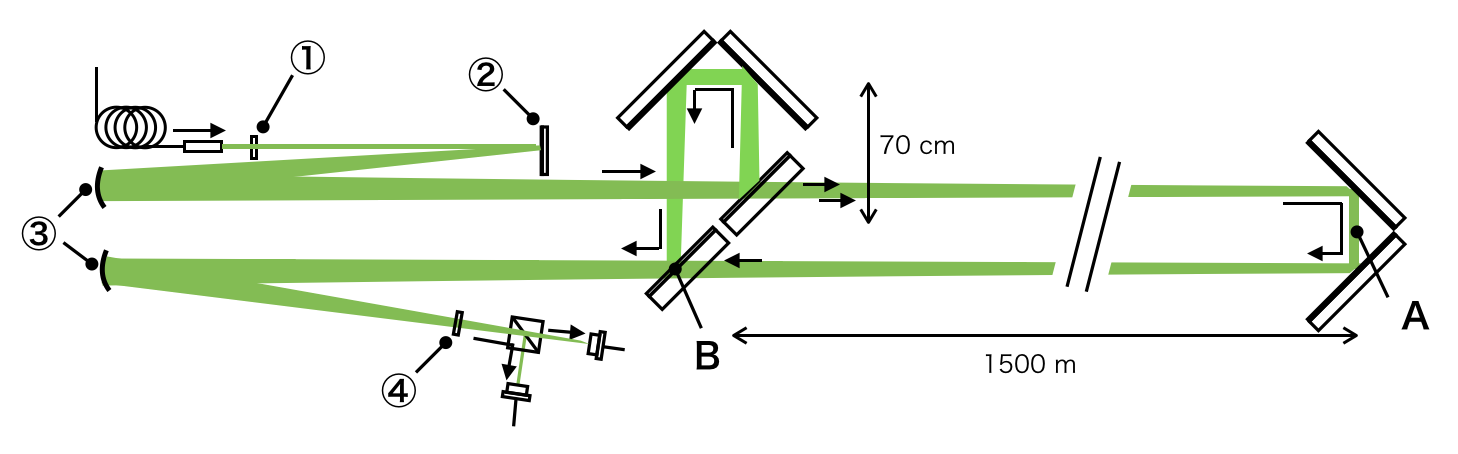
\includegraphics[width=14cm]{./img_chap4/img416.png}
    \caption{Schematic optics layout}{(1) A collimator lens for input beam. (2) A flat mirror for steering mirror. (3) Two concave mirrors with a radius of curvature of $9.8\,\mathrm{m}$ for mode matching. (4) A collimator lens for output beam. The waist of the beam is at the end reflector at point A. Two reflected on the reflectors are combined at point B.}\label{img:img416}
  \end{center}
\end{figure}

\begin{figure}[p]
  \begin{minipage}[b]{0.5\hsize}
    \begin{center}   
      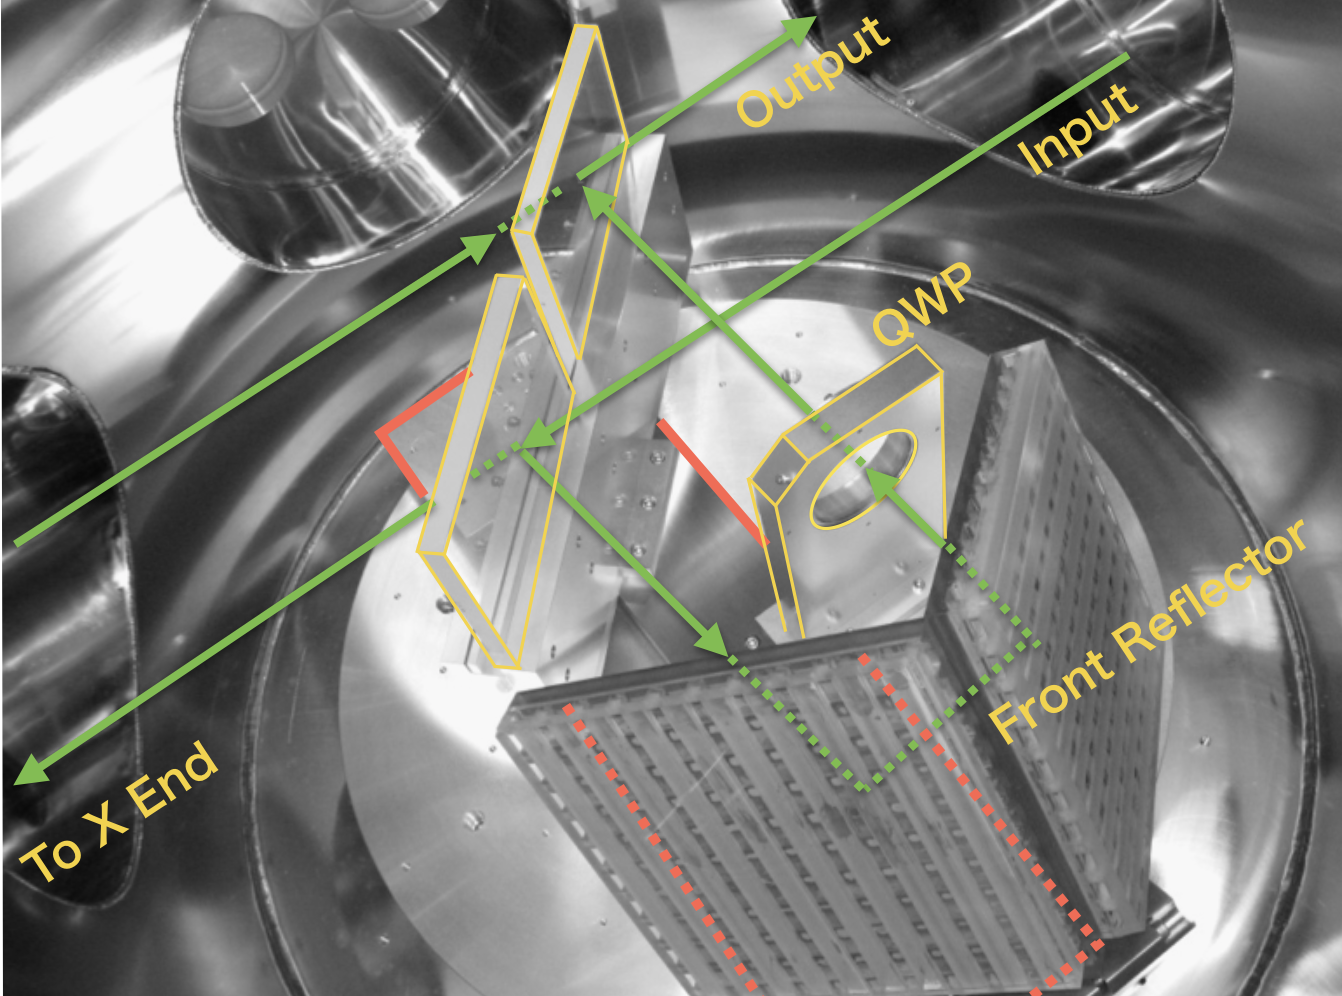
\includegraphics[width=7cm]{./img_chap4/img418.png} % ファイル重い
      %
\includegraphics[width=7cm]{./img.png}
      \subcaption{Core optics in the front vacuum chamber. }\label{img:img418}
    \end{center}
  \end{minipage}\hspace{0.1cm}
  \begin{minipage}[b]{0.5\hsize}
    \begin{center}   
      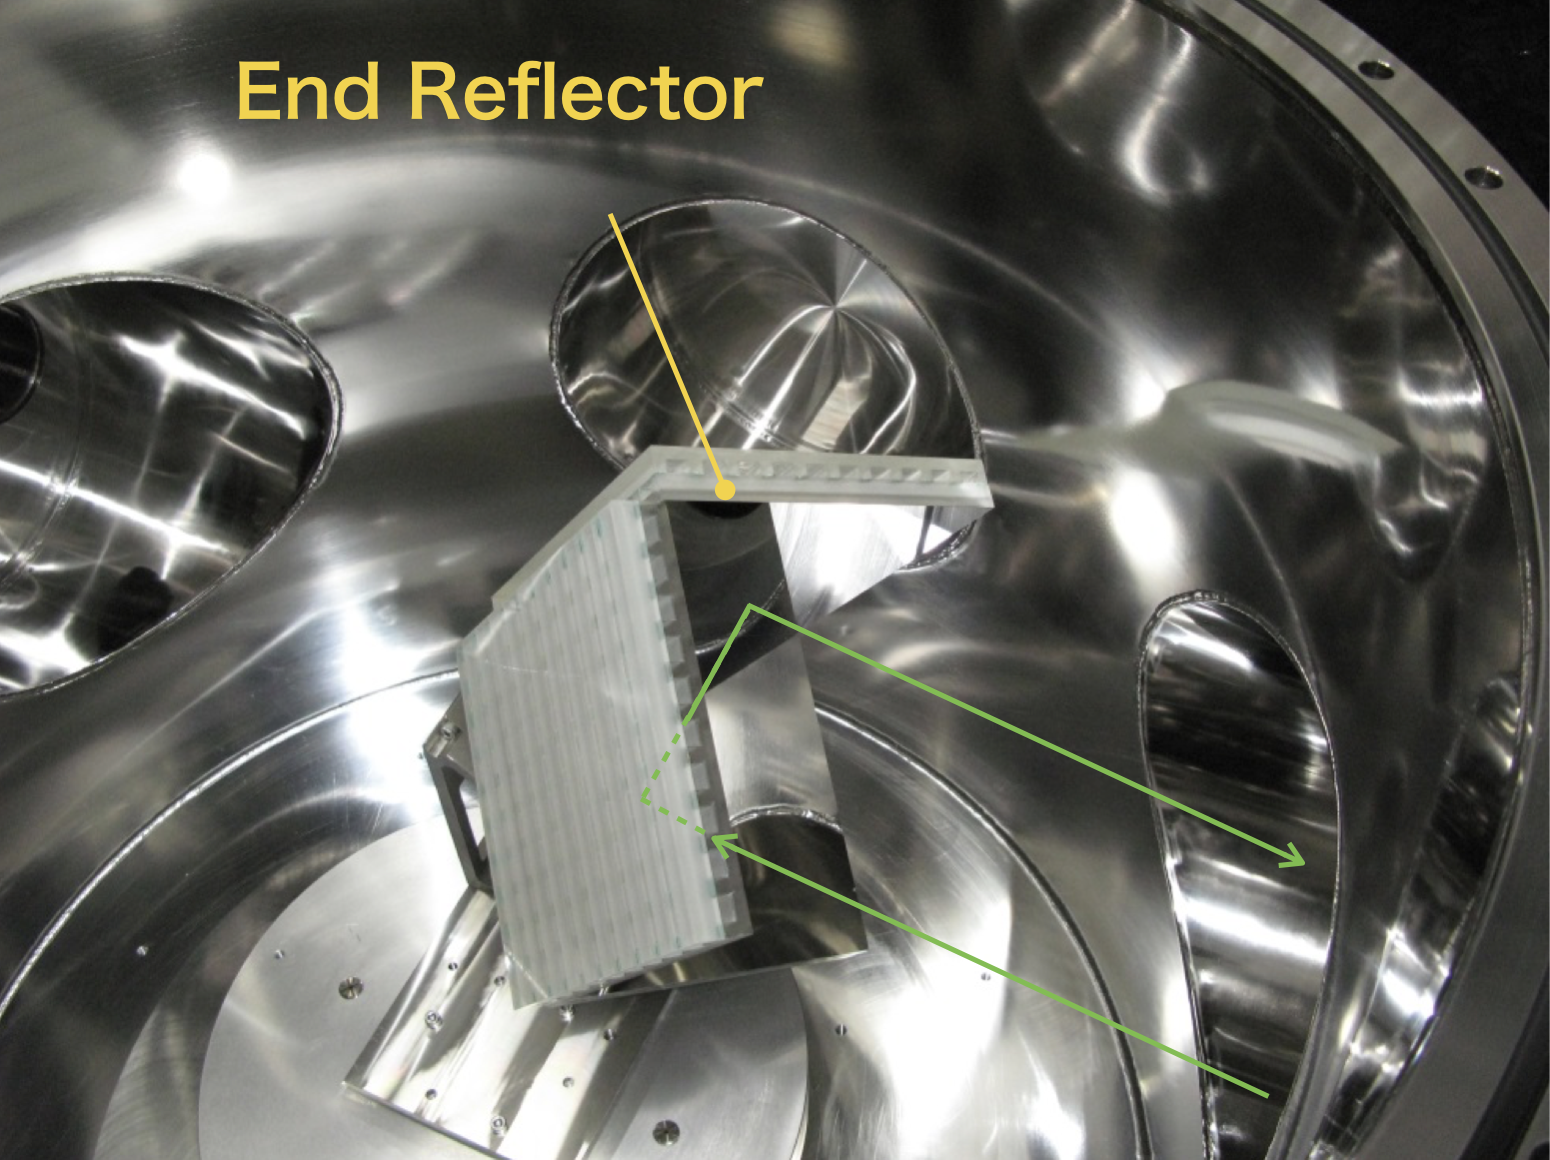
\includegraphics[width=7cm]{./img_chap4/img419.png} %ファイル重い
      %
\includegraphics[width=7cm]{./img.png}      
      \subcaption{Core optics in the end vacuum chamber. }\label{img:img419}
    \end{center}
  \end{minipage}
  \caption{The picture of the core optics.}  
\end{figure}


\subsection{Input Output Optics}
Input output optics is used for matching the beam profile of the input laser and the interferometer in order to interfere as shown in Figure  \ref{img:img416}. The output beam from the laser incident to beam splitter (BS) using (1) a colimator, (2) steering mirror, and (3) concave mirrors in order to be the beam waist at the end reflector. The reflected beams from each reflector are re-combine at the Point B, and this interferered light is incidents to the photo detector through the anothoer concave mirror and colimator. The mode matching is described in reference \cite{miyo2017baseline}.


\subsection{Core Optics}
The core optics of the Michelson interferometer are composed of two reflectors and beam splitter (BS). 


\subsection{Frequency Stabilized Laser} \label{sec:sec135}
As mentioned in \cref{sec:123}, because the frequency noise of the laser is limits the sensitivity of the strain measurement, the GIF interferometer use the frequency stabilized laser utilizing the iodine absorption line \cite{araya2002iodine}. The control diagram of the frequency stabilization system is shown in Figure \ref{img:img417}. This control is a feedback system in order to reduce the error signal of the laser frequency and the frequency of the iodine absorption line. The error signal is obtained by PDH method from the absorption signal that is a doppler free signal by using the pump and prob light \cite{snyder1980high}.
\begin{figure}[h]
  \begin{center}   
    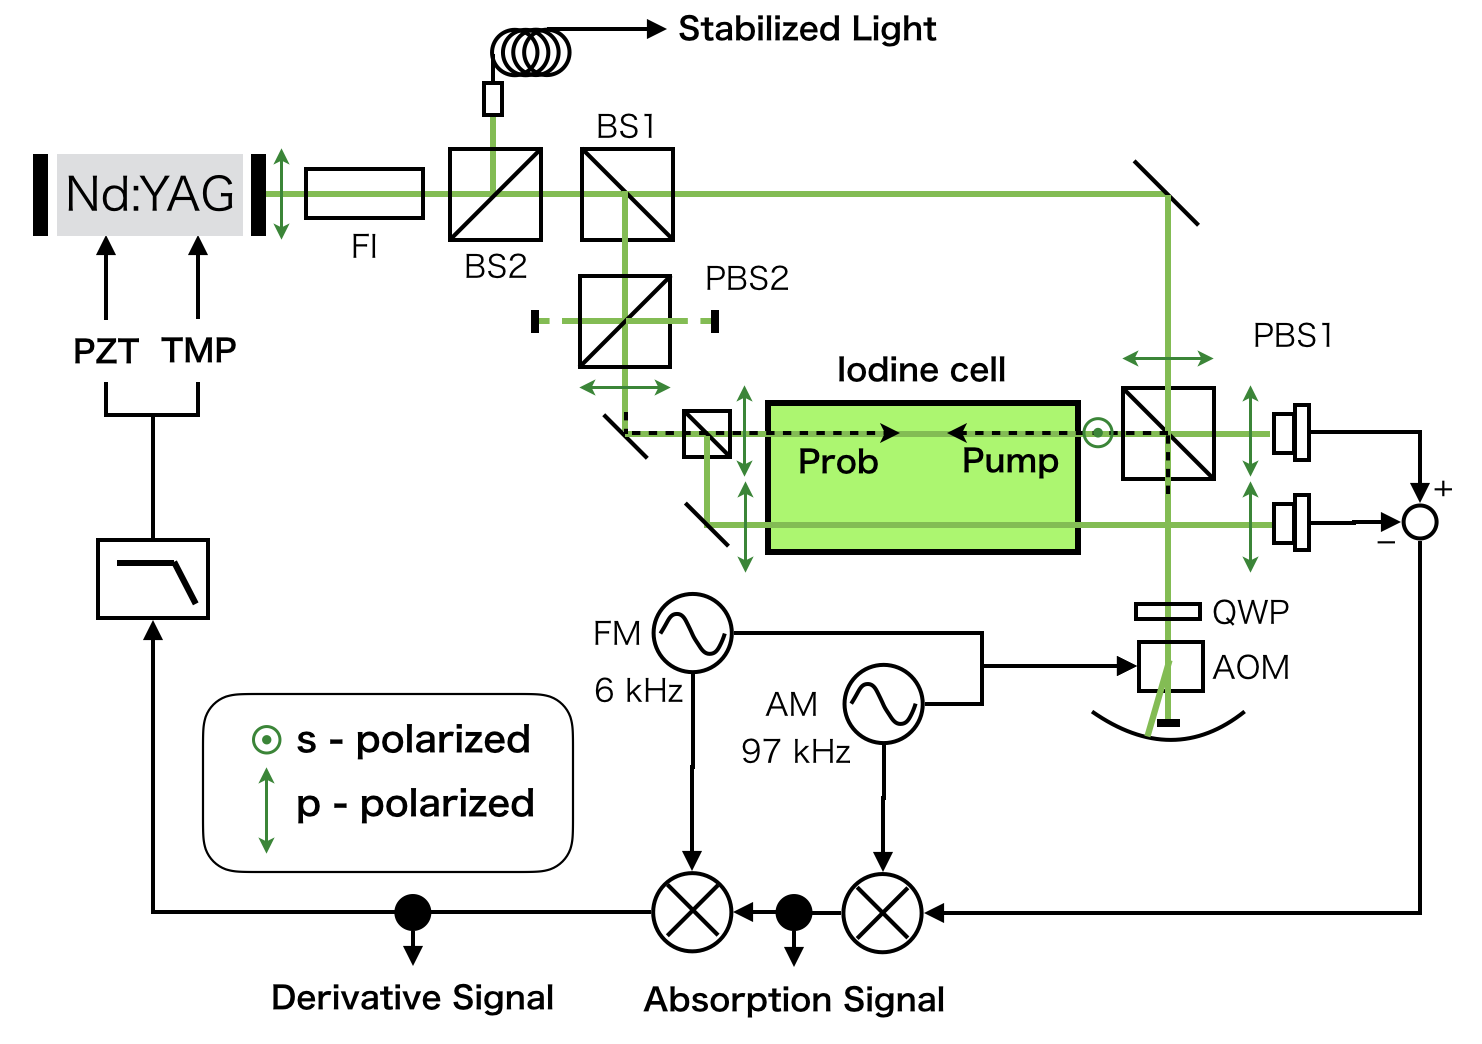
\includegraphics[width=12cm]{./img_chap4/img417.png}
    \caption{Schematic diagram of the frequency-stabilization system of the GIF main laser.}\label{img:img417}
  \end{center}
\end{figure}




\section{Realtime Data Aquisition System} \label{sec:sec44}
Essentialy, the GIF is an independent instrument from the KAGRA not to interfere each other. Therefore, the data aquisition system of eachs were developed independently. However, in order to use the GIF strainmeter for baseline compensation system, we need to impliment the GIF system into the KAGRA system. 

In this section, the realtime data aquisition system is described.
In the section \cref{sec:141}, we describe the quadrature phase detection scheme for obtain the optical phase propotional to the strain on X-arm baseline. In this scheme, we need the elipse fitting to obtain the optical phase. In the section \cref{sec:142}, the realtime data aquisition system is described. This system process the fitting below $1\,\mathrm{msec}$.

\subsection{Quadrature Phase Fringe Detection} \label{sec:141}
\begin{figure}[h]
  \begin{center}
    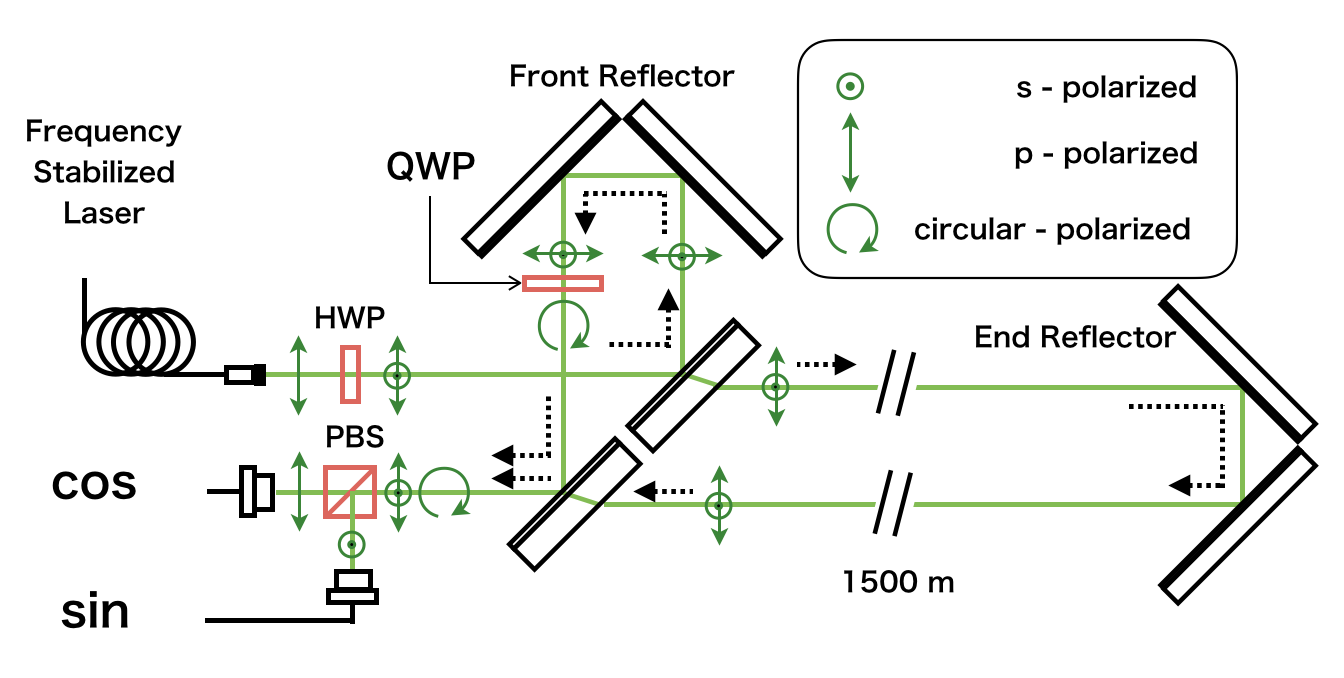
\includegraphics[width=13.0cm]{./img_chap4/img413.png}
    \caption{Quadrature interferometer used in the GIF strainmeter.}\label{img:img413}
  \end{center}
\end{figure}
We use the quadrature phase fringe detection to measure the length change of the baseline with wide dynamic range \cite{bobroff1993recent}. The optical layout for the detection is shown in Figure  \ref{img:img413}. A half-wave plate (HWP) produces a p-polarization and s-polarization. A quator-wave plate (QWP) delay the optical phase of the s-polarized light with 90 degree against to the another. As a result, one can obtain the quadrature phase fringes.

The quadrature phase fringes are detected by two photo detectors, these can be represented as 
\begin{eqnarray}
  x(t) &=& x_0 + b \cos(\phi(t)), \label{eq:eq450b} \\
  y(t) &=& y_0 + a \sin(\phi(t)+\delta), \label{eq:eq450a}  
\end{eqnarray}
where $x$ and $y$ are the two voltage outputs from the detectors, $a$ and $b$ are the amplitudes of these fringe signals, $x_0$ and $y_0$ are the offsets, $\phi$ is optical phase, and $\delta$ is the phase offsets from imperfections \cite{zumberge2004resolving}. Here, the optical phase $\phi$ is given by
\begin{eqnarray}
  \phi = \arctan {\frac{\bar{Y}}{\bar{x}}} \label{eq:eq440c}
\end{eqnarray}
where 
\begin{eqnarray}\label{eq:eq440a} 
  \bar{Y} = \left(\frac{\bar{y}-\bar{x}\sin{\delta}}{\cos{\delta}}\right), \\
  \bar{x} = \frac{x-x_0}{b}\,\,\mathrm{and}\,\,\bar{y} = \frac{y-y_0}{a}. \label{eq:eq440b}
\end{eqnarray}
According to Eq.(\ref{eq:eq400}), if these parameters are given in at time $t$, the optical phase $\phi(t)$ is obtained.


\subsection{Realtime Data Processing} \label{sec:142}
All the PD signals of the GIF are taken by the analog-digital-converter (ADC) and processed in the KAGRA digital system, which is the same as LIGO \cite{bork2001overview}. The ADC converts the analog signal to the digital signal with 16 bit and $2^{16}\,\mathrm{Hz})$ sampling frequency. All the digital signals are simultaneous sampled in the digital system. 

The realtime culculation model in the KAGRA system is shown in Figure  \ref{img:img420}. To reduce the calculation cost, the digital signal in this model is downsampled to $2^{14}\,\mathrm{Hz}$. This realtime model has three main functions; the elipse fitting function, the strain calclator function, and the unwrap function. These functions are described below.
\begin{figure}[h]
  \centering
  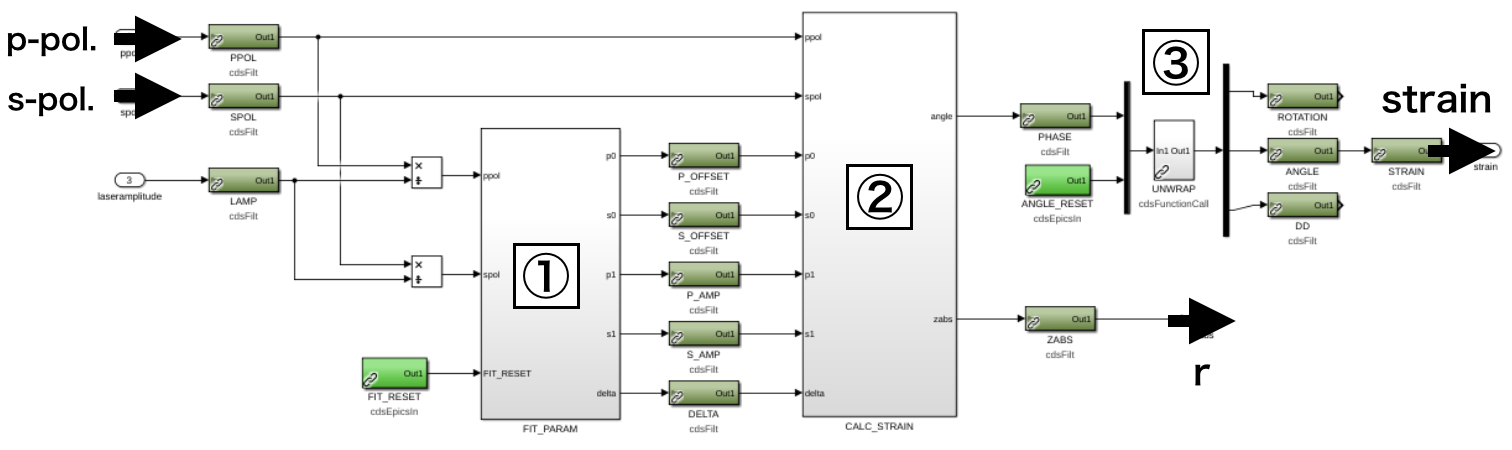
\includegraphics[width=15.0cm]{./img_chap4/img420.png}
  \caption{Realtime calculation model of the phase calculator of GIF. (1) the elipse fitting function (2) the strain calclator function (3) the unwrap function.}\label{img:img420}
\end{figure}

\begin{figure}[h]
  \centering
  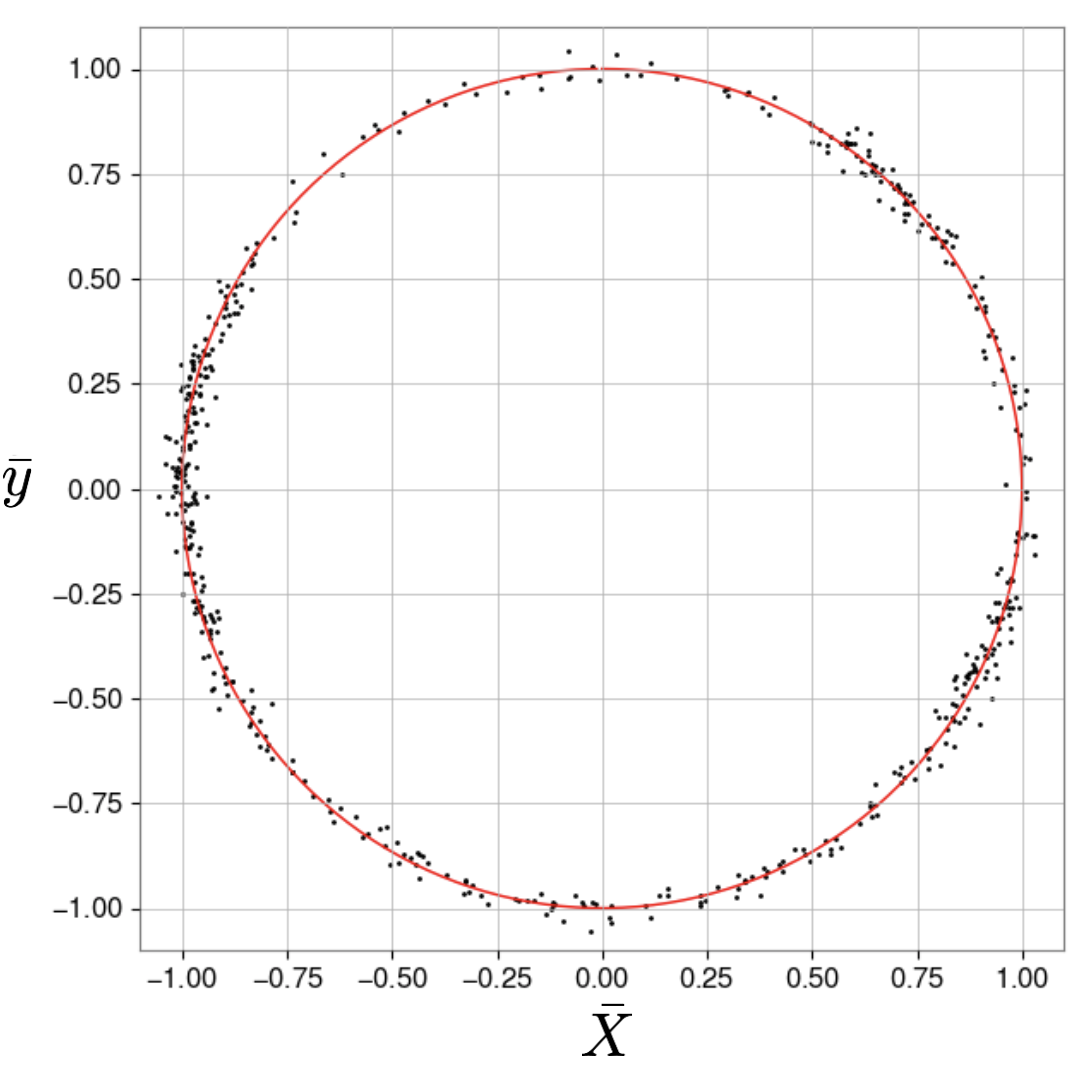
\includegraphics[width=10cm]{./img_chap4/img440.png}
  \caption{Fitting the elipse curve to the Lissajous figure. $\bar{X}$ and $\bar{y}$ are defined in Eq.(\ref{eq:eq440a},\ref{eq:eq440b}), respectively. } \label{img:img440}
\end{figure}

\subsubsection{Elipse fitting function}
This function is for obtainning the five elipse parameters in Eq.(\ref{eq:eq450a,eq:eq450b}) by fitting the elipse curve to the Lissajous figure drawn by two PD signals. The function calculates these parameters using the least-square method with 512 data points of each two PD signal. These data points are moved every sampling time.

\subsubsection{Strain calculator function}
This function calculate the optical phase using the elipse parameters based on Eq.(\ref{eq:eq440c}). For example, Figure  \ref{img:img440} shows the fitted curve (red line) and the data points (black dots). As described above, the optical phase $\phi$ is a angle of the data point. This optical phase is depend on the power ratio $\bar{y}/\bar{x}$ and the phase offset $\delta$ because the phase is given by
\begin{eqnarray}
  \phi = \frac{\bar{y}}{x}\frac{1}{\cos{\delta}} - \tan{\delta}.
\end{eqnarray}
This means that the changes of the power ration and the phase offset are the noise of the optical phase measurement. In particular, the power ratio is sensitive at the PBS which divids the interfered two polarized lights. For this reson,  we covered this location with small house to protect winds disturbed by passengers. On the other hand, the phase offset has small fluctuation because the QWP is installed in the vacuum chamber.

Although the calculation of the optical phase by measuring the angle is not affected by the input power changes, the signal noise ratio will worse in less input power. We also monitor the quality of the calculation using a parameter;
\begin{eqnarray}
  r = \sqrt{\bar{X}^2+{\bar{y}^2}}.
\end{eqnarray}

\subsubsection{Unwrap function}
This function unwrap the optical phase calculated by the phase calculator function and return the continuous phase proportional to strain, because the atan2 function used in the phase calculator return between from $-\pi$ to $\pi$. 

\section{Summary of the Chapter} 
In this chapter, the following items are described:
\begin{itemize}
\item Geophysics interferometer (GIF) installed in parallel to the KAGRA X-arm has a strainsensitivity of $\sim\,10^{-12}$.
\item The advantage of GIF is the wide dynamic range and operation without active alignment control on the mirrors. This feature realizes the long-term stable operation.
\end{itemize}
